\documentclass{article}
\usepackage[a4paper, margin=1.5cm]{geometry}
\usepackage{amsmath, amsfonts, amssymb}
\usepackage{listings}
\usepackage{multicol}
\usepackage{titlesec}
\usepackage{fancyhdr}
\usepackage{xcolor}
\usepackage{tikz}
\usepackage{fourier-orns}
\usetikzlibrary{shapes.geometric, arrows.meta, positioning}

\renewcommand\headrule{%
\hrulefill
\raisebox{-2.1pt}
{\quad\decofourleft\decotwo\decofourright\quad}%
\hrulefill}

\definecolor{codegreen}{rgb}{0,0.6,0}
\definecolor{codegray}{rgb}{0.5,0.5,0.5}
\definecolor{codepurple}{rgb}{0.58,0,0.82}
\definecolor{backcolour}{rgb}{0.95,0.95,0.92}

\lstdefinestyle{mystyle}{
    backgroundcolor=\color{backcolour},   
    commentstyle=\color{codegreen},
    keywordstyle=\color{magenta},
    numberstyle=\tiny\color{codegray},
    stringstyle=\color{codepurple},
    basicstyle=\ttfamily\footnotesize,
    breakatwhitespace=false,         
    breaklines=true,                 
    captionpos=b,                    
    keepspaces=true,                 
    numbers=left,                    
    numbersep=5pt,                  
    showspaces=false,                
    showstringspaces=false,
    showtabs=false,                  
    tabsize=2
}

\lstdefinestyle{plainstyle}{
  backgroundcolor={},   
  frame=none,           
  numbers=none,         
  basicstyle=\ttfamily, 
  breaklines=true,      
  showstringspaces=false, 
}

\lstset{style=mystyle}
\titleformat{\section}[hang]{\normalfont\Large\bfseries}{\thesection.}{1em}{}
\title{C Programming Exercise Solution for Beginner}

\begin{document}
  \pagestyle{fancy}
  \fancyhf{}
  \fancyhead[LE]{\nouppercase{\rightmark\hfill\leftmark}}
  \fancyhead[RO]{\nouppercase{\leftmark\hfill\rightmark}}
  \fancyfoot[LE,RO]{\hfill\thepage\hfill}
  \author{
		Student Name: Fauzy Madani \\ 
		SMKN 1 GARUT \\
		Pengembangan Perangkat Lunak Dan Gim }

  \maketitle

  \tableofcontents

  \clearpage

  \begin{abstract}
  i'm currently learning C and planning to improve my \LaTeX Skill. so i came up with this idea. This is only for my learning purpose. doing C problem while writing the solution and
  my approach/solution to a \LaTeX Note. i'm gonna explain my approach to solve given problem.
  \end{abstract}

  \section{Calculate product of two integers}
  
  Write a C program that accepts two integers from the user and calculates the product of the two integers.
  Test Data :
  
  \begin{lstlisting}[style=plainstyle]
  > Input the first integer: 25
  > Input the second integer: 15
  Expected Output:
  > Product of the above two integers = 375
  \end{lstlisting}
  
  \subsection{Solution}
  \begin{lstlisting}[language=C, caption=Defining required Variable]
    #include <stdio.h>

    #define HEIGHT 7
    #define WIDTH 5
    #define RADIUS 6
    #define M_PI 3.14159265358979323846
    
    // global scope variable declaration
    int num1, num2, result;
  \end{lstlisting}
  
  when you declaring a number using a \texttt{\#define}, It has no type. It is a simple text substitution. although PHI is already defined by C itself, but i found on a stack overflow thread, they were defining PHi with \texttt{\#define}.
  this kind of problem can be tackled easyly by creating a separate \textit{function} outside of \texttt{main()} function, and declaring those variable using \textit{a global scope variable} for efficiency and avoiding conflict within other function. 
  while defining a global scope variable, i'm creating a function to calculate the integers:
  \begin{lstlisting}[language=C, caption=function]
  void CalculateTwoIntegers(int num1, int num2){
    result = num1 + num2;
    printf("The result is: %d\n", result);
  }
  \end{lstlisting}

  \subsection{Pros And Cons}
  
  by storing a number in \texttt{\#define}, it's not the best practice in the modern C. because as i said, \textbf{It has no data types, hard to debug, there's no scope, and etc.} 
  i'd reccomend using a \texttt{const} variable instead. for example: \texttt{const double PI = 3.1415926535;}. a \texttt{\#define} is more suitable for storing a macro rather than a number for mathematical operation unless you know what are you doing.
  
  \section{Calculate average weight for purchases} 
  
  Write a C program that accepts two item's weight and number of purchases (floating point values) and calculates their average value.
  for example: 
  
  \begin{lstlisting}[style=plainstyle]
  Weight - Item1: 15
  No. of item1: 5
  Weight - Item2: 25
  No. of item2: 4
  Expected Output:
  Average Value = 19.444444
  \end{lstlisting}
  
  \subsection{Solution}
  
  by using math shit for this problem, i've figured out using average value for calculating the result, we can implement this solution to our code:
  
  \begin{equation}
  \text{Average Value} = \frac{(w_1 \times n_1) + (w_2 \times n_2)}{n_1 + n_2}
  \label{eq:average-value}
  \end{equation}

  \vspace{2pt}
  
  As shown in Equation~\ref{eq:average-value}, By creating a separate function and declaring the required variable first using \texttt{double} data types, finally we can implement the math formula above
  to our code solution.
  \begin{lstlisting}[language=C, caption=Code Solution]
  void CalculatePurchases(){
    double wi1, ci1, wi2, ci2, resultDouble;
    
    printf("Enter Weight for item 1: ");
    scanf("%lf", &wi1);

    printf("Enter Weight for ci1: ");
    scanf("%lf", &ci1);

    printf("Enter Weight for weight item 2: ");
    scanf("%lf", &wi2);

    printf("Enter Weight for ci2: ");
    scanf("%lf", &ci2);

    resultDouble = ((wi1 * ci1) + (wi2 * ci2)) / (ci1 + ci2);
    printf("The result is %lf\n", resultDouble);
  } 
  \end{lstlisting}
  
  \textbf{\textit{Why does \texttt{scanf()} require to use \& ?}} well, It needs to change the variable. Since all arguments in C are passed by value you need to pass a pointer if you want a function to be able to change a parameter.
  Here's a super-simple example showing it:

  \begin{lstlisting}[language=C, caption=scanf example]
    void nochange(int var) {
    // Here, var is a copy of the original number. &var != &value
    var = 1337;
    }
    void change(int *var) {
        // Here, var is a pointer to the original number. var == &value
        // Writing to `*var` modifies the variable the pointer points to
        *var = 1337;
    }
    int main() {
        int value = 42;
        nochange(value);
        change(&value);
        return 0;
    }
  \end{lstlisting}
  
  C function parameters are always "pass-by-value", which means that the function scanf only sees a copy of the current value of whatever you specify as the argument expression.
  In this case \&i is a pointer value that refers to the variable i. scanf can use this to modify i. If you passed i, then it would only see an uninitialized value, which (a) is UB, (b) is not sufficient information for scanf to know how to modify i.

  \section{Print employee ID and monthly salary}
  
  Write a C program that accepts an employee's ID, total worked hours in a month and the amount he received per hour. Print the ID and salary (with two decimal places) of the employee for a particular month.
  Test Data :
  
  \begin{lstlisting}[caption=Input, style=plainstyle]
    Input the Employees ID(Max. 10 chars): 0342
    Input the working hrs: 8
    Salary amount/hr: 15000
    > Expected Output:
    Employees ID = 0342
    Salary = U\$ 120000.00 
  \end{lstlisting}
  
  for this problem, we need thee type of data:
  \begin{enumerate}
    \item{ID, it can be \texttt{char, int, or an array}. depends on the problem.} 
    \item{working hours, with \texttt{int} data types.}
    \item{Salary amount, \texttt{float} or \texttt{double} is fine.}
  \end{enumerate}
  by using this math formula to calculate the result:
  
  \begin{equation}
  Salary = hoursworked \times rateperhour
  \label{eq:salary}
  \end{equation}

  \subsection{Solution}

  Thus, as shown in equation \ref{eq:salary}, we can implement this math formulae to our code. in my opinion, my approach is too common but i believe this is an efficient way. and more importantly, i don't care about your opinion.
  \begin{lstlisting}[language=C, caption=Code Implementation]
    int working_hours, id;
    double salary_amount_per_hour;

    float CalculateWorkingHours()
    {
      printf("Enter employees ID: ");
      scanf("%d", &id);
      
      printf("Enter working hours: ");
      scanf("%d", &working_hours);
    
      printf("Enter salary_amount per hours: ");
      scanf("%lf", &salary_amount_per_hour);
    
      return working_hours * salary_amount_per_hour;
    }
  \end{lstlisting}
  by creating a separate function, i'm using \texttt{float} to return a float data types when the function is called. if you want to return a more accurate data types
  i'd reccomend using \texttt{double} types. but in this case we're not performing a complex math operation so \texttt{float} is fine for me.
  Thus, i called the function and store it as a variable in order to print the result. 
  \begin{lstlisting}[language=C, caption=Call the function]
    int main()
    {
      float salary = CalculateWorkingHours();
      printf("Salary = U\$ %.2f\n", salary);
      return EXIT_SUCCESS;
    }
  \end{lstlisting}

  \clearpage

  \section{Find the maximum of three integers}
  
  Write a C program that accepts three integers and finds the maximum of three. Test Data :
  
  \begin{lstlisting}[style=plainstyle]
    Input the first integer: 25
    Input the second integer: 35
    Input the third integer: 15
    Expected Output:
    Maximum value of three integers: 35 
  \end{lstlisting}

  my approach for this problem is by creating three integer variable and then store it as an array. for this problem, we can use 
  an algorithm called \textit{Linear search algorithms}. 

  \vfill\null

  \subsection{Linear Search in Mathematical Form}
  
  
  Linear search works by sequentially checking each element in the list until the desired value is found or the end of the list is reached.
  Given an array $A = [a_1, a_2, \dots, a_n]$ and a target value $x$, linear search looks for an index $i$ such that:
  
  \[
  a_i = x, \quad \text{where } 1 \leq i \leq n
  \]
  
  If found:
  
  \[
  f(x, A) =
  \begin{cases}
  i, & \text{if } a_i = x \text{ for some } i \in \{1, \dots, n\} \\
  -1, & \text{if } x \notin A
  \end{cases}
  \]
  
  \textbf{Number of Comparisons:}
  \[
  \begin{aligned}
  C_{\text{best}}(n) &= 1 \\
  C_{\text{worst}}(n) &= n \\
  C_{\text{avg}}(n) &= \frac{n + 1}{2}
  \end{aligned}
  \]
  
  \textbf{Time Complexity:}
  
  \[
  \begin{aligned}
  O_{\text{best}} &= O(1) \\
  O_{\text{worst}} &= O(n) \\
  O_{\text{avg}} &= O(n)
  \end{aligned}
  \]

  In Linear Search, we iterate over all the elements of the array and check if it the current element is equal to the target element. If we find any element to be equal to the target element, then return the index of the current element. Otherwise, if no element is equal to the target element, then return -1 as the element is not found. Linear search is also known as sequential search.
  
  \begin{center}
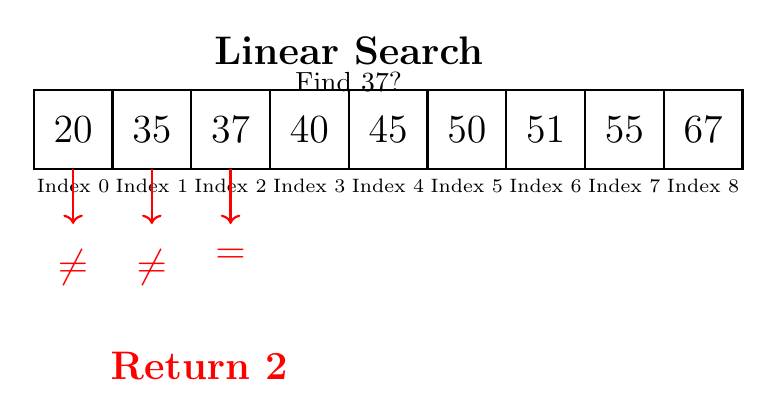
\begin{tikzpicture}[arrow/.style={->, red, thick}]
  % Title
  \node at (4, 4.5) {\Large \textbf{Linear Search}};
  \node at (4, 4.1) {\normalsize Find 37?};

  % Draw array boxes
  \foreach \val [count=\i from 0] in {20,35,37,40,45,50,51,55,67} {
    \draw[thick] (\i*1,3) rectangle ++(1,1);
    \node at (\i*1 + 0.5, 3.5) {\Large \val};
    \node[below] at (\i*1 + 0.5, 3) {\scriptsize Index \i};
  }

  % Arrows showing comparison
  \draw[arrow] (0.5,3) -- +(0,-0.7);
  \node[below, red] at (0.5,2.1) {\Large $\neq$};

  \draw[arrow] (1.5,3) -- +(0,-0.7);
  \node[below, red] at (1.5,2.1) {\Large $\neq$};

  \draw[arrow] (2.5,3) -- +(0,-0.7);
  \node[below, red] at (2.5,2.1) {\Large $=$};

  \node[below=1.2cm, red] at (2.1,2.0) {\Large \textbf{Return 2}};
  \end{tikzpicture}
  \end{center}

  \subsection{Solution}

  we're declaring a global scope variable first to avoid getting an error.
  to implement the \textit{linear search algorithms}, we can create a function outside of \texttt{main}:

  \begin{lstlisting}[language=C, caption=findMax function]
    // Function to find the maximum using linear traversal
    int findMax(int array[], int size) {
        int max = array[0];  // Start from the first element
    
        for (int i = 1; i < size; i++) {
            if (array[i] > max) {
                max = array[i];  // Update max if current is greater
            }
        }
    
        return max;
    }

  int main() {
    int num1, num2, num3;

    // Input from user
    printf("Enter num1: ");
    scanf("%d", &num1);

    printf("Enter num2: ");
    scanf("%d", &num2);

    printf("Enter num3: ");
    scanf("%d", &num3);

    // Create array
    int array[] = {num1, num2, num3};
    int n = sizeof(array) / sizeof(array[0]);

    // Find and print the maximum value
    int maxVal = findMax(array, n);
    printf("The maximum value is: %d\n", maxVal);

    return EXIT_SUCCESS;
  }
 
  \end{lstlisting}

  \subsection{Some Notes}

  \begin{multicols}{2}
    This program does not implement a classic linear search in the strictest sense, because it isn’t looking for the index of a specific target value provided by the user. Instead, it performs a maximum value search within a fixed-size array by linearly traversing each element from the beginning to the end. During this traversal, the algorithm compares each element with the current maximum value and updates the maximum if a larger value is found. This approach still falls under the category of linear search in a broader sense, because it uses the same principle: going through the array one element at a time without skipping or using any advanced techniques like binary search. The time complexity remains O(n), where n is the number of elements in the array, which is identical to the complexity of a standard linear search. So, while the purpose differs (finding the maximum instead of locating a specific value), the method used aligns closely with linear search behavior.
  \end{multicols}

\end{document}
